\documentclass[11pt,a4paper]{article}

\usepackage[margin=1.1in]{geometry}
\usepackage{amsmath,amssymb,amsthm,mathtools}
\usepackage[T1]{fontenc}
\usepackage{microtype}
\microtypesetup{expansion=false}
\usepackage{tikz}
\usetikzlibrary{positioning,arrows.meta,calc,fit,backgrounds,patterns}
\usepackage{booktabs}
\usepackage{listings}
\usepackage{stmaryrd}
\usepackage[hidelinks]{hyperref}
\usepackage{enumitem}

\theoremstyle{plain}
\newtheorem{theorem}{Theorem}
\newtheorem{proposition}[theorem]{Proposition}
\newtheorem{lemma}[theorem]{Lemma}
\newtheorem{corollary}[theorem]{Corollary}
\newtheorem{conjecture}[theorem]{Conjecture}
\theoremstyle{definition}
\newtheorem{definition}[theorem]{Definition}
\newtheorem{observation}[theorem]{Observation}
\theoremstyle{remark}
\newtheorem{remark}[theorem]{Remark}

\newcommand{\rt}{\mathsf{rho}}
\newcommand{\Ctx}{\mathrm{Ctx}}
\newcommand{\Lrn}{\mathcal{L}}
\newcommand{\Nsp}{\mathcal{N}}
\newcommand{\Met}{\Nsp_{\mathrm{met}}}
\newcommand{\Src}{\Nsp_{\mathrm{src}}}
\newcommand{\Prb}{\Nsp_{\mathrm{prb}}}
\newcommand{\Mat}{\Nsp_{\mathrm{mat}}}
\newcommand{\sep}[2]{\mathbin{\big|^{#1}_{#2}}}
\newcommand{\Th}{\mathrm{Th}}
\newcommand{\fn}{\mathrm{fn}}
\newcommand{\Merge}{\bowtie}
\newcommand{\qq}[1]{@#1}

\lstdefinestyle{rho}{
  basicstyle=\ttfamily\footnotesize,
  keywordstyle=\bfseries,
  commentstyle=\itshape,
  morekeywords={new,in,for,contract,match,if,else,true,false,Nil,where,and,or,not,
                exists,forall,nu,TOP},
  morecomment=[l]{//},
  columns=fullflexible,
  breaklines=true,
  breakatwhitespace=false,
  showstringspaces=false,
  frame=none,
  xleftmargin=1em
}
\lstset{style=rho}

\title{\textbf{Composing Learners}\\[0.4em]
\large Populations as namespaces, parallel composition as the operator,\\
and the ecological relations that typed overlap generates}
\author{L. G. Meredith\\ \small F1R3FLY.io}
\date{August 1, 2026}

\begin{document}
\maketitle

\begin{abstract}
Two companion notes model learning as the loop the scientific method describes, run by a
computation with a finite and conserved token supply in an environment made of other
computations~\cite{scientist}, and instantiate that model on a solved adversarial game so that
its claims can be checked against answers the reader already holds~\cite{game}. In both, the
learner is an individual and the population is what rescues it: confinement says an individual's
incremental revisions cannot leave the ball its early commitments placed it in, and recombination
across a lineage is the only escape.

This note takes the population as the learner. A learner is a distribution over a population of
scientists, of mortal computations holding no hypothesis, and of resource reservoirs; because
that population is carried by a family of names manufactured by quotation, a learner
\emph{is} a namespace, described by a name predicate rather than enumerated. Learners then
compose by parallel composition, and the whole content of the composition is what their
namespaces share.

Four things follow. Disjointness of namespaces is exactly factorisation of the distribution, so
composition is strictly monoidal at zero grade and the lax structure map elsewhere \emph{is} the
interaction; the deviation from strictness is therefore a measurement rather than a caveat. A
single grade is too coarse: the namespace of a learner is typed---metabolic, source, probe,
mating---and grading separately over each recovers the classical table of ecological relations as
sign conditions rather than importing it. Conservation makes cooperation and competition
structurally unlike: tokens are conserved and formulae are not, so mutualism is available only
over the probe namespace and competition only over the metabolic and source ones. And
disjointness is not stable, because names manufactured independently may coincide; modular
composition is purchasable, and the price is a naming discipline that roots each learner's
namespace at its own quotation.

We then measure. A second environment---Nim---is laddered exactly by the same method and
schedule as~\cite{game}, and it inverts that note's headline: in Nim$(1,2,3)$ marginal return
\emph{rises} up the ladder and the complete theory is the best purchase on it, where in
noughts-and-crosses returns collapse and the complete theory is dominated. Whether truth is
affordable is a property of the environment, not of the learner, and composition puts several
such answers under one conserved budget. Composing the two over a single rate-limited
reservoir gives a closed form: each learner retains exactly the fraction $c_{\text{other}} /
(c_{\text{self}}+c_{\text{other}})$ of the inquiry it could afford alone. The dilution is
regressive---it costs the unfinished science $66.9\%$ of its affordable depth and the finished
one nothing---and it is delivered without either learner perceiving, modelling, or touching the
other. Finally, exhaustion of a shared reservoir forces the grading vector to change, and only
the learner that was confined retains the apparatus to change it. We close on the observation
that composition is the exit from the heat death of~\cite{game}: a population that has solved its
science stops eating, and the cheapest way to make it eat again is to compose it with a learner
whose namespace it has not solved.
\end{abstract}

\tableofcontents

\section{Introduction}

\subsection{Why the unit moves up}

The mortal scientist of~\cite{scientist} is an individual: a term with a metabolic channel, a
hypothesis in guard position, and a walk on the relaxation lattice. Twice in that note the
individual turns out to be the wrong unit. Corollary~31 there observes that destructive assay
leaves an individual-level hypothesis worthless after its own first test, so the \emph{subject} of
a hypothesis must be a namespace rather than a specimen. And Proposition~13 observes that an
ultrametric walk of short steps never leaves the ball it began in, so the \emph{holder} of a
hypothesis cannot repair a shallow commitment; \S12 of that note supplies recombination, and
\S17.2 states plainly that a population is required rather than preferred.

The worked example makes both visible on numbers~\cite[\S9]{game}. The corner-opening
mutant that invades the resident population differs from it by a revision of distance $2^{-1}$,
is unreachable to any individual by deepening, and is free to a lineage because the cost falls on
an offspring holding no confirmations to invalidate.

So the individual is already not the unit of learning; the lineage is. This note asks what happens
when the lineage is not the unit either.

\subsection{The move, stated once}

A learner is a distribution over a population: scientists, mortal computations holding no
hypothesis, and resource reservoirs. That population is carried by names, and by Proposition~2
of~\cite{game} those names are manufactured by quotation rather than drawn from a stock of
atoms, so the family is generated by a decidable predicate and can be \emph{described}. Hence a
learner is a namespace, in the sense the hypothesis language already uses for the subject of a
hypothesis.

Learners compose by parallel composition, because in this calculus there is nothing else for
composition to be. When the namespaces are disjoint the composed learners have non-interacting
capabilities. When they overlap they can interact internally, and that interaction includes both
cooperation and competition.

\begin{remark}[The knower and the known become one kind of thing]
This is the observation we would lead with. Corollary~31 of~\cite{scientist} forces the
\emph{object} of inquiry to be a namespace; the present move makes the \emph{subject} of inquiry
one as well. The two sides of the cut are then described in the same vocabulary, by the same name
predicates, at the same prices. That is not tidiness for its own sake: it is what makes a
composed learner able to hold a hypothesis about its own components, and what makes the
distinction between an internal interaction and an external one a matter of where one draws the
cut rather than a matter of sort. Remark~40 of~\cite{scientist} said trophic type is a fact about
the cut. The same is now true of learnerhood.
\end{remark}

\subsection{What we are claiming, and what we are not}

We claim that composition of learners is parallel composition on terms, union on namespaces, and
\emph{undetermined} on distributions; that the determination of the third is exactly the content
of the interaction, and that it factors precisely when the namespaces are disjoint; that a single
grade of separation is too coarse and a typed vector of grades recovers the ecological relations
rather than importing them; that under conservation cooperation and competition are structurally
different rather than opposite in sign; that non-interference is an observation and not a
guarantee unless purchased; and that a composite's phase is not a function of its parts' phases,
which we exhibit on exact numbers.

We do not claim to have proved a monoidal-category theorem: \S\ref{sec:comp} states the
comparison map and the conditions for it to be invertible, and leaves the coherence to the
open problems. We do not claim the access-rate model of \S\ref{sec:dilution} is canonical; it is
one modelling choice, flagged as such, and the alternative is worked. As in~\cite{game}, guards
below are written in the ideal logic and the current interpreter accepts only the arithmetic and
pattern fragment of the \texttt{where} clause; occurrences that specify rather than perform a
check are marked.

\section{What is imported}

We recapitulate only what the argument uses, and refer to~\cite{scientist,game,classifier} for
the rest.

\paragraph{The cut, and three grades of access.}
A world is $W \equiv S \mid E$. Computations are ontologically isolated, so $E$ is other
computations, and what $S$ can come to know of $E$ is bounded above by $E$'s context-labelled
bisimulation class. Access comes in three grades and no more: \emph{perception}, structural
predicates evaluated at the surface, priced by a schedule $\kappa_{\mathrm{sense}}(d)$ monotone
in formula depth; \emph{interaction}, the context-labelled modalities $\langle K_j\rangle$,
costing a rendezvous per step; and \emph{reflection}, the name predicate $@\varphi$ applied to
names $S$ already holds, cheap because it passes through no surface.

\paragraph{The logic is generated, and there is no restriction.}
Feeding the presentation of the rho calculus to the OSLF family yields one structural connective
per term former, one context-labelled modality per rewrite rule and redex position, and---because
$\mid$ carries an associative--commutative theory---a separating conjunction. A name is a quoted
process, so $n \models @\varphi \iff n = @P$ with $P \models \varphi$: this is namespace
logic~\cite{nslogic}, in which one describes a namespace by a property rather than enumerating
it. Following~\cite[\S2]{game} we treat \texttt{new} as sugar and drop the hidden-name
quantifier: freshness is manufactured by quotation, and graded separation is graded over a
\emph{described namespace} rather than over a restriction vector,
\[
  P \models \varphi \sep{\Nsp}{k} \psi
  \iff
  P \equiv Q \mid R,\ Q \models \varphi,\ R \models \psi,\
  \bigl|\, \fn(Q) \cap \fn(R) \cap \Nsp \,\bigr| = k .
\]
Everything below that a modal logic could not do is done with $\sep{\Nsp}{k}$, and
\S\ref{sec:typed} turns on the choice of $\Nsp$.

\begin{proposition}[Freshness by quotation, {\cite[Prop.~2]{game}}]\label{prop:fresh}
Let $P$ be a process and $C[-]$ any context with $C[P] \neq P$. Then $@C[P] \notin n(P)$. Hence a
name fresh in $P$ is manufactured by quoting any term properly containing $P$, with no registry
and no consultation.
\end{proposition}

\paragraph{Conservation and the game.}
Tokens are conserved: $\sigma + \kappa = \sigma_0 = \Theta$, with $\sigma$ held in live stacks
and $\kappa$ migrated into the record. There is no primary producer. Under the internalising
encoding $\llbracket - \rrbracket : \mathcal{C}(\rt) \to \rt$ a located stack becomes a message
at a metabolic channel $m_P$, and harvest is an ordinary receipt on $m_P$ performed by someone
else; the predatory contexts are exactly the non-image contexts holding a metabolic
name~\cite[Thm.~25]{scientist}. A \emph{game} is a choice of admitted context class $\mathcal{A}$
with $\llbracket \mathcal{C}(\rt)\text{-}\Ctx \rrbracket \subseteq \mathcal{A} \subseteq
\rt\text{-}\Ctx$.

\paragraph{Sources and prey.}
The trophic distinction is an access profile, not a sort~\cite[\S11.2]{scientist}: a
\emph{source} is a persistent emitter, rate-limited by being a single contract, non-exclusive,
non-adaptive, and exhaustible; a \emph{prey} is a linear send, exhaustible, exclusive, and
adaptive. By Proposition~41 there, a source-feeder's inquiry converges and a prey-feeder's never
does.

\paragraph{The hypothesis space, and confinement.}
Beneath the characteristic formula $\chi_P$ sits a lattice of progressively weaker formulae
obtained by forgetting conjuncts; revision is a walk on it, the metric is the $\nu$-stratified
ultrametric $d(\varphi,\psi) = 2^{-n}$, and distance, modal depth, and cost are one graded
structure. Confinement (Proposition~13 of~\cite{scientist}) says a walk whose steps are all
shorter than $2^{-n}$ never leaves the ball of radius $2^{-n}$ it began in; cost-monotonicity
(Proposition~15) says the escaping move is the expensive one; and bounded branching
(Proposition~18) with its corollary \emph{poverty is confining} says the number of siblings a
scientist may evaluate is its stack divided by the cost of checking one.

\paragraph{Ecologies as a fibration.}
A configuration is a partition of $\Theta$ across loci together with a structural assignment; an
ecology is a configuration with a distribution over reachable configurations. The assignment of
ecologies to theories is a fibration rather than a functor, with a canonical section given by
taking cost as the weight map, and functoriality requires logic-preserving morphisms because the
senses are structural~\cite[\S15]{scientist}. The present note is largely an argument that this
fibration wants a tensor.

\section{The learner}\label{sec:learner}

\subsection{Three layers, and the distribution is one of them}

What we have been calling a learner has three components, and it is worth separating them before
asking what composition does, because composition acts differently on each.

\begin{enumerate}[label=(\roman*)]
\item \textbf{A population.} A term: a parallel composition of scientists, of mortal
computations holding no hypothesis, and of reservoirs. This is an object of the calculus.
\item \textbf{A namespace.} The family of names the population carries---metabolic channels,
source channels, probe channels, mating channels---described by a name predicate rather than
listed, which by Proposition~\ref{prop:fresh} is available because the names are manufactured
from material the population already holds.
\item \textbf{A distribution.} A weighting on the configurations reachable from the population,
in the sense of~\cite[\S13]{scientist}: the microcanonical ensemble at fixed $\Theta$, sampled by
the construction of~\cite{gillespie-note}.
\end{enumerate}

We take the third to be part of the learner rather than a decoration on it. The alternative---a
learner is the population, and the distribution is a decoration indexed over it---would put
composition in the base of the fibration of~\cite[\S15]{scientist}, where it is uninformative:
two populations composed in the base are just two populations. Putting the distribution inside
the learner puts composition in the total space, which is where the interaction lives.

\begin{definition}[Learner]\label{def:learner}
A learner is a triple $\Lrn = (P, \Nsp, \mu)$ with $P$ a $\rt$ term, $\Nsp$ a name predicate
satisfied by exactly the names $P$ carries in the sense of Definition~\ref{def:typed} below, and
$\mu$ a distribution over the configurations reachable from $P$ at total $\Theta_{\Lrn} =
\sum \sigma_i(0)$. We write $\Nsp(\Lrn)$ and $\mu(\Lrn)$ for the components.
\end{definition}

\begin{remark}[The population is not a bag of learners]
Definition~\ref{def:learner} does not say the population is a set of individual learners composed
somehow. It says the population, weighted, \emph{is} the learner, and that individual scientists
inside it are components with no special status---exactly as a lineage in~\cite[\S12.10]{scientist}
is a learner without any of its members being the learner. The nesting is real and the note uses
it: \S\ref{sec:units} shows the three units of learning are distinguished by nothing but the
revision distance each can reach.
\end{remark}

\section{Composition}\label{sec:comp}

\subsection{One operator, three actions}

\begin{definition}[Composition]\label{def:comp}
For learners $\Lrn_1 = (P_1,\Nsp_1,\mu_1)$ and $\Lrn_2 = (P_2,\Nsp_2,\mu_2)$,
\[
  \Lrn_1 \mid \Lrn_2 \;:=\; \bigl(\,P_1 \mid P_2,\ \ \Nsp_1 \vee \Nsp_2,\ \ \mu_{12}\,\bigr),
  \qquad \Theta_{\Lrn_1 \mid \Lrn_2} = \Theta_{\Lrn_1} + \Theta_{\Lrn_2},
\]
where $\Nsp_1 \vee \Nsp_2$ is the disjunction of the two name predicates and $\mu_{12}$ is the
distribution over configurations reachable from $P_1 \mid P_2$.
\end{definition}

On the first component the operator is the calculus' own parallel composition: associative and
commutative up to structural congruence, free, and adding nothing. On the second it is
disjunction of predicates, which is again free, and is where describing rather than enumerating
pays---one does not have to compute a union of two sets of names, one takes an $\vee$ of two
formulae. On the third the operator is not determined by its arguments at all. That is the
entire subject of this section.

\begin{proposition}[Conservation composes, and only conservation does]
$\Theta$ is additive under composition, and it is the only quantity in~\cite[\S13]{scientist}
that is. The order parameters are not: $\iota$, the fraction of $\Theta$ internal to scientists,
is a stack-weighted mean of the parts' values, and $\delta$, the mean concealment depth of
external stacks, is not a function of the parts' values at all, because each learner's members
become candidate subjects for the other and enter the other's mean.
\end{proposition}

\begin{proof}[Proof sketch]
Additivity of $\Theta$ is immediate from the ledger law and the fact that composition mints
nothing. For $\iota$, write $\iota_i = \sigma^{\mathrm{sci}}_i / \Theta_i$; then
$\iota_{12} = (\sigma^{\mathrm{sci}}_1 + \sigma^{\mathrm{sci}}_2)/(\Theta_1+\Theta_2)$, the
weighted mean. For $\delta$, the mean is taken over the external stacks \emph{available to} a
learner, and $P_2$'s stacks are external to $P_1$ and were not in $P_1$'s index set. So
$\delta_{12}$ depends on the depth at which each learner's stacks lie relative to the other's
senses, a quantity computed from the pair and not held by either.
\end{proof}

That $\delta$ is a property of the pair is the first sign that composition is not going to be
innocent, and \S\ref{sec:phase} makes it a measurement.

\subsection{Disjointness is factorisation}

\begin{theorem}[Factorisation]\label{thm:factor}
Let $\Lrn_1, \Lrn_2$ be learners and let $\Nsp = \Nsp_1 \vee \Nsp_2$. The following are
equivalent.
\begin{enumerate}[label=(\arabic*)]
\item $P_1 \mid P_2 \models \top \sep{\Nsp}{0} \top$ with the split at $P_1, P_2$: the two
namespaces share no name.
\item No reduction of $P_1 \mid P_2$ has its redex spanning the two parands.
\item $\mu_{12} = \mu_1 \otimes \mu_2$: the composite's distribution is the product of the
parts'.
\end{enumerate}
\end{theorem}

\begin{proof}[Proof sketch]
$(1)\Rightarrow(2)$: the rho calculus has one interaction rule, and it requires a send and a
receipt on structurally equal names. A redex spanning the parands therefore witnesses a name in
$\fn(P_1) \cap \fn(P_2) \cap \Nsp$, contradicting $k=0$. $(2)\Rightarrow(3)$: with no spanning
redex, every step of $P_1\mid P_2$ is a step of one parand in a context that does not participate,
so the reachable configurations are pairs of independently reachable configurations, and the
weight of a pair is the product of the weights since the cost of a step is charged to the parand
taking it and the ledger is additive. $(3)\Rightarrow(1)$: if a name is shared, some
configuration in which the corresponding rendezvous has fired has weight not equal to the product
of its marginals---the two parands' stacks after such a step are correlated by the transfer.
\end{proof}

\begin{remark}[Why this is the right statement]
Theorem~\ref{thm:factor} is what makes ``the namespaces are disjoint'' worth saying. Disjointness
of \emph{names} is a syntactic condition; independence of \emph{distributions} is the thing one
actually wants when composing learners, because it is what licenses reasoning about each in
isolation. The theorem says the syntactic condition is exactly the probabilistic one, and the
graded separation $\sep{\Nsp}{k}$ measures the gap when it fails. We know of no way to say this
without a spatial layer: a purely behavioural logic cannot state the split at all, which is
\cite[Rem.~5]{classifier} arriving in a new place.
\end{remark}

\subsection{The lax structure map is the interaction}

Composition of learners is a candidate monoidal structure on the total space of the fibration
$\pi : \mathrm{Eco} \to \mathrm{GSLT}_{\mathcal{C}}$ of~\cite[\S15]{scientist}, with unit the
empty learner $(\mathbf{0}, \bot, \delta_{\varnothing})$. The obvious question is whether the
canonical section $s$---cost as the weight map---is monoidal, and the answer is no, in a way we
think is more useful than a yes.

\begin{proposition}[Laxity, and what its defect measures]\label{prop:lax}
There is a comparison morphism
\[
  \lambda_{\Lrn_1,\Lrn_2} \;:\; s(\Lrn_1) \otimes s(\Lrn_2) \longrightarrow s(\Lrn_1 \mid \Lrn_2)
\]
sending a pair of independently sampled trajectories to the interleaving in which no spanning
redex fires. It is an isomorphism if and only if the grade is zero, and in general it is not
epi: the configurations in the image are exactly those reachable without interaction. The
deviation---the mass $\mu_{12}$ assigns outside the image of $\lambda$---is the probability that
the composite does something neither part could do.
\end{proposition}

\begin{proof}[Proof sketch]
Existence: the non-interacting interleavings of two independent trajectories are reachable in the
composite, and their weights are the products, since costs are additive. Iso at $k=0$: Theorem
\ref{thm:factor}. Failure of surjectivity at $k>0$: a spanning redex is enabled and fires with
positive rate under any weight map assigning positive weight to enabled steps, and the resulting
configuration is not a product of independently reachable ones.
\end{proof}

\begin{remark}[The good news is that laxity is a number]
Conjecture~82 of~\cite{scientist} guesses that the induced map on distributions is only lax and
that the natural target is distributions ordered by stochastic dominance. Composition sharpens
the guess into something one can compute: the defect of $\lambda$ is the total interaction, and
$\sep{\Nsp}{k}$ resolves it by which names carry it. Cooperation and competition are then not two
phenomena to be modelled but two \emph{signs} of one measured quantity, and \S\ref{sec:coop} says
which sign each namespace can carry.
\end{remark}

\section{Typed overlap: the grading vector}\label{sec:typed}

\subsection{One grade is not enough}

The game note's Proposition~7 is the lesson in miniature. There the connective was
$\sep{\Nsp}{0}$ and the concept was \emph{fork}; grading over line names made the formula true of
pairs of threats sharing a gap, which are not forks, and grading over square names made it exact.
The choice of $\Nsp$ was not a parameter of the encoding but the whole content of it.

At the level of learners the same demand recurs, and the namespace of a learner is not
homogeneous. A shared metabolic channel and a shared probe channel are both ``an overlap of one
name'' and they are not remotely the same relation.

\begin{definition}[Typed namespaces]\label{def:typed}
For a learner $\Lrn$ with population $P$, the namespace $\Nsp(\Lrn)$ decomposes into four
sub-namespaces, each given by a name predicate:
\begin{itemize}[itemsep=2pt]
\item $\Met(\Lrn)$, the \emph{metabolic} names: the channels at which $P$'s components hold their
stacks, in the sense of~\cite[Def.~21]{scientist};
\item $\Src(\Lrn)$, the \emph{source} names: the channels of persistent emitters $P$ draws on,
the access profile of~\cite[Def.~39]{scientist};
\item $\Prb(\Lrn)$, the \emph{probe} names: the channels on which $P$'s scientists install
assays, which by~\cite[\S12.6]{scientist} are both-type channels supporting dialogue of depth at
least two;
\item $\Mat(\Lrn)$, the \emph{mating} names: the channels on which genomes are disclosed and
recombined.
\end{itemize}
\end{definition}

\begin{definition}[Grading vector]\label{def:vector}
For learners $\Lrn_1,\Lrn_2$ the grading vector is
\[
  \mathbf{k}(\Lrn_1,\Lrn_2) \;=\;
  \bigl(k_{\mathrm{met}},\, k_{\mathrm{src}},\, k_{\mathrm{prb}},\, k_{\mathrm{mat}}\bigr),
  \qquad
  k_{\tau} = \bigl|\, \fn(P_1)\cap \fn(P_2) \cap \Nsp_{\tau} \,\bigr| ,
\]
the componentwise grade at which $P_1 \sep{\Nsp_\tau}{k_\tau} P_2$ holds. Composition is
\emph{non-interacting} when $\mathbf{k} = \mathbf{0}$.
\end{definition}

\begin{figure}[t]
\centering
\resizebox{\textwidth}{!}{%
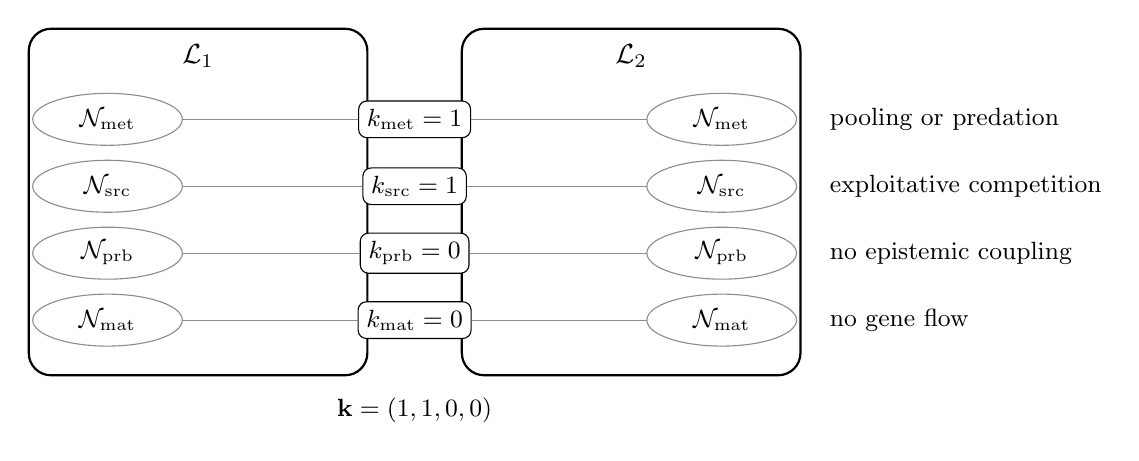
\begin{tikzpicture}[scale=1.0]
\definecolor{lgrey}{gray}{0.55}
% left learner
\draw[thick, rounded corners=8pt] (-4.9,-2.2) rectangle (-0.6,2.2);
\node at (-2.75,1.85) {$\Lrn_1$};
% right learner
\draw[thick, rounded corners=8pt] (0.6,-2.2) rectangle (4.9,2.2);
\node at (2.75,1.85) {$\Lrn_2$};
% four lobes each
\foreach \y/\lab in {1.05/{$\Met$}, 0.2/{$\Src$}, -0.65/{$\Prb$}, -1.5/{$\Mat$}} {
  \draw[lgrey] (-3.9,\y) ellipse (0.95 and 0.33);
  \node[font=\small] at (-3.9,\y) {\lab};
  \draw[lgrey] (3.9,\y) ellipse (0.95 and 0.33);
  \node[font=\small] at (3.9,\y) {\lab};
}
% overlaps
\node[draw, fill=white, rounded corners=3pt, font=\small, inner sep=3pt] (m) at (0,1.05)
  {$k_{\mathrm{met}}=1$};
\node[draw, fill=white, rounded corners=3pt, font=\small, inner sep=3pt] (s) at (0,0.2)
  {$k_{\mathrm{src}}=1$};
\node[draw, fill=white, rounded corners=3pt, font=\small, inner sep=3pt] (p) at (0,-0.65)
  {$k_{\mathrm{prb}}=0$};
\node[draw, fill=white, rounded corners=3pt, font=\small, inner sep=3pt] (t) at (0,-1.5)
  {$k_{\mathrm{mat}}=0$};
\foreach \n/\y in {m/1.05, s/0.2, p/-0.65, t/-1.5} {
  \draw[lgrey] (-2.95,\y) -- (\n); \draw[lgrey] (\n) -- (2.95,\y);
}
\node[font=\small, align=left, anchor=west] at (5.15,1.05) {pooling or predation};
\node[font=\small, align=left, anchor=west] at (5.15,0.2) {exploitative competition};
\node[font=\small, align=left, anchor=west] at (5.15,-0.65) {no epistemic coupling};
\node[font=\small, align=left, anchor=west] at (5.15,-1.5) {no gene flow};
\node[font=\small] at (0,-2.65) {$\mathbf{k} = (1,1,0,0)$};
\end{tikzpicture}}
\caption{Two composed learners and their grading vector. A single scalar $k$ would report
``$2$'' and say nothing; the typed vector says the two share a metabolic channel and a
reservoir, cannot read each other's assays, and cannot interbreed. Those are four independent
dials and \S\ref{sec:relations} reads the ecological relation off them.}
\label{fig:vector}
\end{figure}

\subsection{The relations, derived}\label{sec:relations}

The point of typing the overlap is that the classical table of ecological relations then falls
out as sign conditions on the components, rather than being imported as a taxonomy. Write
$\Delta_i$ for the change in learner $i$'s expected residual life under composition relative to
isolation.

\begin{table}[t]
\centering
\footnotesize
\begin{tabular}{@{}llll@{}}
\toprule
overlap & relation & $(\Delta_1,\Delta_2)$ & mechanism \\
\midrule
$\mathbf{k}=\mathbf{0}$ & neutralism & $(0,0)$ & Theorem~\ref{thm:factor}: $\mu$ factors \\
$k_{\mathrm{src}}>0$ only & exploitative competition & $(-,-)$ &
  dilution of a finite reserve (\S\ref{sec:dilution}) \\
$k_{\mathrm{met}}>0$, asymmetric & predation & $(+,-)$ &
  harvest as a receipt \cite[Def.~23]{scientist} \\
$k_{\mathrm{met}}=1$, pooled & mutualism (metabolic) & $(+,+)$ &
  the composite of \cite[Prop.~44]{scientist} \\
$k_{\mathrm{prb}}>0$, one-way & commensalism (epistemic) & $(+,0)$ &
  reading a surface another paid for \\
$k_{\mathrm{prb}}>0$, two-way & mutualism (epistemic) & $(+,+)$ &
  \S\ref{sec:coop}: formulae are not conserved \\
$k_{\mathrm{prb}}>0$, theft & exploitation (epistemic) & $(+,-)$ &
  \cite[\S10]{scientist}: holding a model exposes it \\
$k_{\mathrm{mat}}>0$ & \emph{not composition} & --- &
  \S\ref{sec:merger}: the learners are one \\
\bottomrule
\end{tabular}
\caption{Ecological relations as sign conditions on the grading vector. Nothing in this table is
posited; each row is a consequence already proved in~\cite{scientist} together with a choice of
which $\Nsp_\tau$ carries the overlap.}
\label{tab:relations}
\end{table}

\begin{proposition}[Symbiosis is minimal metabolic overlap]\label{prop:symb}
Let $\Lrn_1 \mid \Lrn_2$ have $k_{\mathrm{met}} = 1$ with the shared name a pooling channel---a
metabolic channel on which both parands both receive and reissue---and $k_\tau = 0$ otherwise.
Then the composite is exactly the construction of~\cite[Prop.~44]{scientist}: two specialists
sharing a metabolic channel, each free to tune its access profile independently, with the yield
pooled. Hence Proposition~43 there, which dominates the mixed strategy for an atom, does not
apply.
\end{proposition}

\begin{remark}[The organism boundary is a grade]
Read with Remark~40 of~\cite{scientist}, Proposition~\ref{prop:symb} says the difference between
``one dual-feeding organism'' and ``two specialists in symbiosis'' is the value of
$k_{\mathrm{met}}$ and where one chooses to draw the cut, not a fact about either. The
endosymbiotic reading is available and we note it without leaning on it~\cite{margulis}: what the
formalism contributes is that the boundary has a number attached to it.
\end{remark}

\begin{proposition}[The grading namespace must be typed]
Let $\Nsp = \Met \vee \Src \vee \Prb \vee \Mat$ and suppose one grades only over $\Nsp$. Then
$\sep{\Nsp}{k}$ cannot distinguish a composite in exploitative competition ($k_{\mathrm{src}}=1$,
rest zero) from one in symbiosis ($k_{\mathrm{met}}=1$, rest zero), since both satisfy
$\sep{\Nsp}{1}$; and the two have opposite signs in Table~\ref{tab:relations}. Hence the vector
of Definition~\ref{def:vector} is not a refinement of convenience.
\end{proposition}

This is the same argument as~\cite[Prop.~7]{game} one level up, and we take the recurrence as
evidence that choosing the grading namespace is where the modelling work in this framework
actually happens.

\section{Cooperation and competition are structurally unlike}\label{sec:coop}

\subsection{Two currencies, one conservation law}

Under Remark~20 of~\cite{scientist} every metabolic transfer is zero-sum: predation is the
purchase of somebody else's remaining time. It follows immediately that cooperation cannot be a
token transfer leaving both parties richer, and one might conclude that a conserved world has no
room for mutualism at all. It does, and the room is in exactly one place.

\begin{observation}[Tokens are conserved; formulae are not]\label{obs:two}
$\Theta$ is fixed and never minted. A formula is a different kind of object: a genome is a
quotation, $@P$ does not reduce, quotation is free while held, and inspection by a name predicate
is grade-three access, the cheapest on the ladder. Nothing forbids two learners from holding the
same formula, and one learner's coming to hold it does not deprive the other. The ecology is
conserved; the epistemics are not.
\end{observation}

\begin{proposition}[No metabolic mutualism]\label{prop:nomet}
Let $\Lrn_1 \mid \Lrn_2$ have $k_{\mathrm{prb}} = k_{\mathrm{mat}} = 0$, so that all overlap is
metabolic or source. Then $\Delta_1 + \Delta_2 \leq 0$, with equality only when no shared name
carries a transfer.
\end{proposition}

\begin{proof}[Proof sketch]
Residual life is stack divided by burn rate. Every step over a shared metabolic or source name
either moves tokens from one parand to the other, which is zero-sum in stack and strictly
negative in aggregate residual life whenever the two burn rates differ, or debits both parands
for the rendezvous, which is negative. Pooling (Proposition~\ref{prop:symb}) is the boundary case
in which the transfer is a loop and the aggregate is unchanged; even there the rendezvous is
metered, so equality requires no transfer at all.
\end{proof}

So the only positive-sum overlap is epistemic, and it has two mechanisms, both already in the
companion notes.

\subsection{Cost relocation, and who is billed}

\begin{observation}[Cooperation is amortised perception]\label{obs:amort}
There are two routes to any predicate about an environment: \emph{read} it, if the environment
has computed it into legible structure, priced by formula depth; or \emph{drive} it, by taking
steps and watching, priced by rendezvous~\cite[\S5.1]{game}. If $\Lrn_1$'s components compute a
predicate into structure standing at a name in $\Prb(\Lrn_1) \cap \Prb(\Lrn_2)$, then $\Lrn_2$
reads at grade one what it would otherwise drive at grade two. The total metering for both
learners to know the predicate falls, and no token has been created.
\end{observation}

Remark~24 of~\cite{game} makes the point that putting threats into the term relocates a cost from
the scientist's budget to the world's, and that the interesting quantity is not whether the work
is done but who is billed for it. Composition is what makes that question have two answers
inside one system. A shared legible surface is stigmergy, and it is the only mechanism by which
two mortal learners in a conserved world can both come out ahead.

\begin{proposition}[Epistemic overlap can be strictly positive-sum]
Let $\varphi$ be a predicate both learners require, costing $\kappa_{\mathrm{drive}}$ to
establish by interaction and $\kappa_{\mathrm{read}}(d) < \kappa_{\mathrm{drive}}$ to read from
structure, and let $\kappa_{\mathrm{write}}$ be the cost to $\Lrn_1$ of computing it into
structure at a shared probe name. Then $\Delta_1 + \Delta_2 > 0$ whenever
\[
  2\,\kappa_{\mathrm{drive}} \;>\; \kappa_{\mathrm{drive}} + \kappa_{\mathrm{write}} +
  \kappa_{\mathrm{read}}(d),
\]
that is, whenever writing once and reading once costs less than driving twice. This is not
available over $\Met$ or $\Src$ by Proposition~\ref{prop:nomet}.
\end{proposition}

\begin{remark}[And the same overlap can be theft]
The mechanism cuts both ways and the notes already say so. Holding a hypothesis requires
exposing it, because a guard is surface, so $\Prb$ overlap that lets $\Lrn_2$ read $\Lrn_1$'s
confirmed structure also lets it read $\Lrn_1$'s theory without experimenting~\cite[\S10]{scientist}.
Whether epistemic overlap is mutualism or exploitation is not settled by the grade; it is settled
by whether the reading learner reciprocates, which is the plagiarism equilibrium left open
as Problem~2 there. What the present framing adds is that the question is well posed as a sign
condition on one component of $\mathbf{k}$.
\end{remark}

\begin{center}
\emph{Cooperation is epistemic; competition is metabolic.}
\end{center}

\section{Non-interference is not stable}\label{sec:stability}

Disjointness of namespaces is the condition under which composition is innocent, so it matters
whether it can be relied upon. It cannot, by default, and the reason is one the companion note
already records for a different purpose.

\begin{proposition}[Disjointness is an observation, not a guarantee]\label{prop:unstable}
Let $\Lrn_1 \mid \Lrn_2$ have $\mathbf{k} = \mathbf{0}$ at some configuration. Because name
manufacture is decentralised and freshness is scope-relative~\cite[Rem.~1]{scientist}, the two
populations may subsequently manufacture structurally equal names at loci private to each. Hence
$\mathbf{k} = \mathbf{0}$ at one configuration does not entail $\mathbf{k} = \mathbf{0}$ at a
successor, and neither learner need have taken any step aimed at the other.
\end{proposition}

\begin{proof}[Proof sketch]
This is Remark~34 of~\cite{scientist}---closure is luck, not construction---together with
Proposition~71 there, that decentralisation makes recombination generative precisely because two
parents may independently hold structurally equal names. What is a source of novelty within a
lineage is a source of unplanned coupling between learners.
\end{proof}

\begin{corollary}[There is no modular composition for free]
One cannot compose two learners and certify non-interference from the parts alone. Certification
requires either a global check at each configuration, which is model checking and is priced, or a
discipline on name manufacture.
\end{corollary}

The discipline exists, it is cheap, and it is the one the board of~\cite[\S4]{game} already uses.

\begin{proposition}[Rooting makes disjointness a theorem]\label{prop:root}
Let $\Lrn_1$ and $\Lrn_2$ manufacture every private name by quoting a term properly containing a
distinguished root $r_1$, respectively $r_2$, with $r_1 \neq r_2$ and neither root occurring in
the other's population. Then no name manufactured by $\Lrn_1$ is structurally equal to a name
manufactured by $\Lrn_2$, and $\mathbf{k}$ is constant along every reduction that does not
introduce a name from outside.
\end{proposition}

\begin{proof}[Proof sketch]
By Proposition~\ref{prop:fresh} a manufactured name is $@C[r_i]$ for a context $C$ with
$C[r_i] \neq r_i$, so it codes a term properly containing $r_i$. Structural equality of
$@C[r_1]$ and $@C'[r_2]$ would give $C[r_1] \equiv C'[r_2]$, and by well-foundedness of the
coding---a name occurring in a term codes a strictly smaller term---this forces $r_1$ to occur in
$C'[r_2]$, contradicting the hypothesis that $r_1$ does not occur in $\Lrn_2$'s population.
\end{proof}

\begin{remark}[Modularity is purchasable, and the price is a naming discipline]
This is the same trick as the board's three name families $@[*b,k]$, $@[*b,\texttt{"m"},k]$,
$@[*b,\texttt{"t"},s]$, which are pairwise disjoint by construction and which is what makes
grading over $\Th_b$ available in the first place. Applied to learners it says: root each
learner's namespace at its own quotation and non-interference becomes a property one can rely on
rather than one one must keep checking. It also says that a learner which \emph{wants} to
interact must import a name from outside its own root, which is a step, which is metered. Under
rooting, every interaction has an identifiable first cause with a price attached---which is a
better situation than the notes have had so far, where accidental coupling was possible and
untraceable.
\end{remark}

\section{Merger}\label{sec:merger}

Overlap in the mating namespace is not a kind of interaction. It is the failure of the two
learners to be two.

\begin{proposition}[Mating overlap collapses the pair]
By~\cite[Prop.~53]{scientist} two computations can recombine exactly at their homologous loci, so
conspecificity is agreement of path sets and reproductive isolation is namespace disjointness. If
$k_{\mathrm{mat}} > 0$ and the shared names are homologous, then genomes cross the boundary,
alleles from each appear in the other's descendants, and after finitely many generations neither
population's namespace is described by its original predicate.
\end{proposition}

\begin{definition}[Merger]\label{def:merger}
The merger $\Lrn_1 \Merge \Lrn_2$ is the learner
\[
  \bigl(\,P_1 \mid P_2,\ \ \Nsp_1 \vee \Nsp_2,\ \ \mu_{\Merge}\,\bigr)
\]
whose distribution ranges over configurations reachable under a recombination discipline admitting
homologous loci \emph{across} the two populations, together with the identification of the two
mating namespaces.
\end{definition}

Merger and composition agree on the first two components of Definition~\ref{def:learner} and
differ on the third, which is precisely why the third had to be part of the learner. As operators
they behave differently in ways worth recording.

\begin{proposition}[Merger is not composition]
Composition is associative and commutative up to $\equiv$ and admits the empty learner as a unit.
Merger is commutative but is neither associative in general---$(\Lrn_1 \Merge \Lrn_2) \Merge
\Lrn_3$ and $\Lrn_1 \Merge (\Lrn_2 \Merge \Lrn_3)$ admit different homology relations, since
homology is not transitive across intermediate path sets---nor unital in the same sense, since
$\Lrn \Merge \mathbf{0}$ imposes an identification that $\Lrn \mid \mathbf{0}$ does not.
Moreover merger is irreversible: no composition of the merged learner recovers the parts, because
the alleles have crossed.
\end{proposition}

\begin{remark}[Why we want it separate]
There is a temptation to treat merger as composition at high $k_{\mathrm{mat}}$ and be done. We
resist it for two reasons. First, the sign structure of Table~\ref{tab:relations} has no entry
for it: merger is not $(+,+)$ or $(+,-)$, because after it there are no two parties to assign
signs to. Second, and more usefully, merger is the operator that changes the \emph{identity} of a
learner while composition changes only its situation, and \S\ref{sec:units} needs that
distinction: a lineage escapes confinement by recombination \emph{within} itself, and a
federation escapes by composition \emph{with} another. Merger is the third thing, and it escapes
by ceasing to be the learner that was confined.
\end{remark}

\section{Phase is not compositional}\label{sec:phase}

Figure~2 of~\cite{scientist} divides the $(\iota,\delta)$ plane into three regions: at low $\delta$
food lies in the open and senses suffice, so a theory is overhead; at high $\iota$ or high
$\delta$ discovery costs more than it returns and everything starves; in between, hypothesis
formation pays. The boundaries are where the foraging inequality changes sign.

\begin{proposition}[Phase is not preserved]\label{prop:phase}
There exist learners $\Lrn_1, \Lrn_2$ each of which lies in the science-pays band in isolation
and whose composite lies outside it. Specifically:
\begin{enumerate}[label=(\alph*)]
\item \emph{Downward, into foraging-suffices.} If $\Lrn_2$'s components lie shallow to $\Lrn_1$'s
senses---$\delta$ small in the pair, which by Remark~3 of~\cite{game} means few plies of
lookahead are needed to model them---then $\Lrn_1$'s cheapest rung dominates its theory-holding
rungs, since the prey is legible without inquiry.
\item \emph{Downward, into starvation.} If composition raises $\iota$ past the upper boundary,
which it does whenever $\Lrn_2$ is stack-rich and reservoir-poor, then no available locus
satisfies the foraging inequality for either party.
\item \emph{Upward, out of starvation.} If $\Lrn_1$ is below its minimum viable endowment and
$k_{\mathrm{met}}=1$ is a pooling channel, then Proposition~\ref{prop:symb} rescues it.
\end{enumerate}
\end{proposition}

The interesting case is none of these three, because all three are couplings a modeller can see
coming. The case worth measuring is the one in which the two learners never perceive each other
at all.

\section{Competitive dilution, measured}\label{sec:dilution}

\subsection{The model, and its one choice}

Take $\mathbf{k} = (0,1,0,0)$: two learners sharing exactly one source name and nothing else.
Neither can perceive the other---no probe name is shared, so no assay of either reaches the
other's surface---neither can harvest the other, and neither can interbreed with it. By
Table~\ref{tab:relations} the relation is exploitative competition, and the only channel of
influence is $\Theta$ itself.

The source is a single contract, hence rate-limited and non-exclusive~\cite[Def.~39]{scientist}.
We must say how the two learners' calls interleave, and this is the note's one genuinely free
modelling choice.

\begin{definition}[Access rate]\label{def:rate}
A learner calling a source completes one assay per $c$ metered units, where $c$ is its expected
metering per assay at the rung it holds. Learners queue at the source as fast as they complete
assays, so learner $i$'s share of the source's payouts is
\[
  s_i \;=\; \frac{1/c_i}{\sum_j 1/c_j}.
\]
\end{definition}

The alternative---equal shares regardless of cost---is defensible if one reads the contract as
serving callers round-robin rather than first-come. We work Definition~\ref{def:rate} and note in
\S\ref{sec:notshown} what changes under the alternative: the dilution survives, the asymmetry
does not.

\begin{proposition}[Competitive dilution]\label{prop:dilution}
Let two learners share one source of reserve $R_0$ paying quantum $q$ per assay, at price $p$
tokens per metered unit, with expected meterings $c_1, c_2$ per assay, both self-funding
($q > p c_i$). Then over the life of the source, learner $i$ receives
\[
  G_i \;=\; \frac{R_0}{q}\cdot \frac{c_{j}}{c_i + c_{j}} \qquad (j \neq i)
\]
assays and accumulates $\Sigma_i = G_i\,(q - p c_i)$. Consequently the number of assays of any
deficit-running rung of cost $c^\ast > q/p$ that learner $i$ can subsequently fund is
\[
  D_i \;=\; \frac{\Sigma_i}{p c^\ast - q}
  \;=\; D_i^{\text{alone}} \cdot \frac{c_{j}}{c_i + c_{j}} ,
\]
so that \emph{each learner retains exactly its own share of the reservoir as a fraction of the
inquiry it could afford in isolation}. The factor is independent of $R_0$, $q$, $p$ and $c^\ast$.
\end{proposition}

\begin{proof}[Proof sketch]
Immediate from Definition~\ref{def:rate}: composition scales $G_i$ by $s_i$ and everything
downstream is linear in $G_i$.
\end{proof}

\begin{corollary}[Dilution is regressive]\label{cor:regressive}
A learner whose best affordable rung is self-funding loses assays but no \emph{depth}, since the
rung it holds needs no surplus. A learner still climbing---whose next rung runs a deficit and must
be funded from accumulated surplus---loses depth in exact proportion to its share. Hence
competition at a shared reservoir costs the unfinished science strictly more than the finished
one, and costs nothing at all to a learner that has stopped.
\end{corollary}

\begin{remark}[Competition is a mechanism of confinement]
Corollary~19 of~\cite{scientist} says poverty is confining: a scientist whose stack affords few
evaluations per move takes the cheapest available move, the cheapest moves are the shortest, and
by Proposition~13 short moves cannot leave their ball. Proposition~\ref{prop:dilution} exhibits
a mechanism of impoverishment that requires no contact whatever. A learner can be confined to a
shallow theory by a competitor that cannot see it, cannot model it, and has no hypothesis about
it---only a name in common. We think this is the most surprising consequence of the composition
operator, and it is the classical competitive exclusion principle~\cite{hardin,tilman} arriving
in an epistemic currency rather than a demographic one.
\end{remark}

\section{The worked example: two games, one wall}\label{sec:worked}

\subsection{A second environment}

The game note laddered noughts-and-crosses and found the complete theory dominated. To compose we
need a second learner, and the second environment should differ in the one respect that matters:
whether its complete theory is affordable.

We take Nim, normal play~\cite{bouton}. The ladder is built by the same method and priced by the
same schedule $\kappa(d) = 2^d$, with the cost of a decision at rung $r$ equal to $|M| \cdot
\sum_{\text{rules } 1..r} \kappa(d_{\text{rule}})$ and $|M|$ the number of legal moves.

\begin{center}
\small
\begin{tabular}{@{}clll@{}}
\toprule
rung & formula added & kind and depth & $\kappa$ \\
\midrule
$0$ & $\top$ & --- & $0$ \\
$1$ & $\exists s.\ \mathrm{One}(s) \wedge \mathrm{Takes}(s)$ & spatial, depth 1 & $2$ \\
$2$ & $\exists s.\ \mathrm{Two} \wedge \mathrm{Equalises}(s)$ & spatial, depth 1 & $2$ \\
$3$ & $\chi_{\mathrm{Nim}} := \exists s.\ \mathrm{NimSum}_0(s)$ & name-level, depth 0 & $1$ \\
\bottomrule
\end{tabular}
\end{center}

Rung 1 says: exactly one heap is nonempty, take it. Rung 2 says: exactly two heaps are nonempty,
equalise them. Rung 3 is Bouton's theorem: move to a position whose nim-sum is zero. All three
are predicates on the heap sizes, read off the reflected structure of the position by a name
predicate; none contains a modality, and rung 3 in particular requires no lookahead at all.

\begin{observation}[The complete theory of Nim is name-level]
$\chi_{\mathrm{Nim}}$ is exact and contains no modality and no fixed point. This is Remark~11 of
\cite{scientist}---a finite theory is complete exactly when the environment's regularity is
structural---in its sharpest available form: Nim's regularity is so structural that its complete
theory sits at depth zero, where noughts-and-crosses needs $\nu X.\forall s.[K_s](\neg
\mathrm{Lost} \wedge \exists t. \langle\langle K_t\rangle\rangle X)$ and nine unfoldings.
\end{observation}

\subsection{The ladder pays, and here it keeps paying}

All figures are exact over all plays, symmetrised over which side moves first, against a
uniform-random opponent, computed by memoised recursion (Appendix~\ref{app:repro}).

\begin{table}[t]
\centering
\small
\begin{tabular}{@{}clrrrrr@{}}
\toprule
rung & added rule & win & loss & cost & $\Delta$win & return \\
\midrule
\multicolumn{7}{@{}l}{\textit{Nim$(3,4,5)$ \quad nim-sum $=2$, an N-position; branching $12$}}\\
$0$ & $\top$ & $0.5000$ & $0.5000$ & $0.0$ & --- & --- \\
$1$ & take-all & $0.6567$ & $0.3433$ & $38.9$ & $+0.1567$ & $+0.00403$ \\
$2$ & equalise & $0.8899$ & $0.1101$ & $80.4$ & $+0.2332$ & $+0.00562$ \\
$3$ & $\chi_{\mathrm{Nim}}$ & $0.9966$ & $0.0034$ & $99.6$ & $+0.1067$ & $+0.00555$ \\
\midrule
\multicolumn{7}{@{}l}{\textit{Nim$(1,2,3)$ \quad nim-sum $=0$, a P-position; branching $6$}}\\
$0$ & $\top$ & $0.5000$ & $0.5000$ & $0.0$ & --- & --- \\
$1$ & take-all & $0.5917$ & $0.4083$ & $15.2$ & $+0.0917$ & $+0.00602$ \\
$2$ & equalise & $0.7958$ & $0.2042$ & $31.4$ & $+0.2042$ & $+0.01262$ \\
$3$ & $\chi_{\mathrm{Nim}}$ & $0.9000$ & $0.1000$ & $38.5$ & $+0.1042$ & $+0.01476$ \\
\bottomrule
\end{tabular}
\caption{Two Nim ladders, exact. Contrast Table~1 of~\cite{game}, where marginal return falls by
more than two orders of magnitude along the ladder and the complete theory is dominated on both
axes. Here return is flat in Nim$(3,4,5)$ and \emph{rising} in Nim$(1,2,3)$, where the complete
theory is the best purchase available.}
\label{tab:nim}
\end{table}

\begin{observation}[Whether truth is affordable is a property of the environment]\label{obs:env}
Three environments, three answers. In noughts-and-crosses $\chi$ costs $679.2$, wins $0.873$, and
is strictly dominated by a name-level heuristic winning $0.918$ at $255.9$. In Nim$(3,4,5)$
$\chi_{\mathrm{Nim}}$ costs $99.6$, wins $0.9966$, and is not dominated: it is more expensive than
the rung below and strictly better. In Nim$(1,2,3)$ it is the best marginal purchase on the whole
ladder, returning $+0.0148$ per metered unit where the rung below returns $+0.0126$ and the rung
below that $+0.0060$. The returns \emph{rise}.
\end{observation}

This is worth stating carefully because it is the hinge of the composition argument. Remark~17 of
\cite{scientist}---yield, not truth---says a lineage under selection drifts toward yield-biased
search wherever yield and discrimination disagree. Table~\ref{tab:nim} shows they do not always
disagree. Whether they do is fixed by the environment: by how much of its regularity is
structural rather than reduction-following (Remark~11 there), and by the branching factor, which
by Proposition~10 of~\cite{game} is the arity of the quantification over redex positions. So
\emph{is truth affordable?} is not a question about scientists. It is a question about worlds, and
composition is the operator that puts two answers into one budget.

\begin{remark}[$\chi$ in a lost position is a fall-through to $\top$]
Nim$(1,2,3)$ has nim-sum zero, so the first player has no move to a zero position and
$\chi_{\mathrm{Nim}}$ fires no rule; the policy falls through to uniform choice. It still wins
$0.800$ as first player because the random opponent errs and the complete theory punishes the
error the moment it appears---but it has nothing to say about how to \emph{provoke} one. As
second player it wins $1.000$. That the complete theory is silent on exploiting a fallible
opponent is Observation~25 of~\cite{game} in a domain where $\chi$ is otherwise cheap and good,
which is some evidence that the phenomenon is about completeness rather than about cost.
\end{remark}

\begin{figure}[t]
\centering
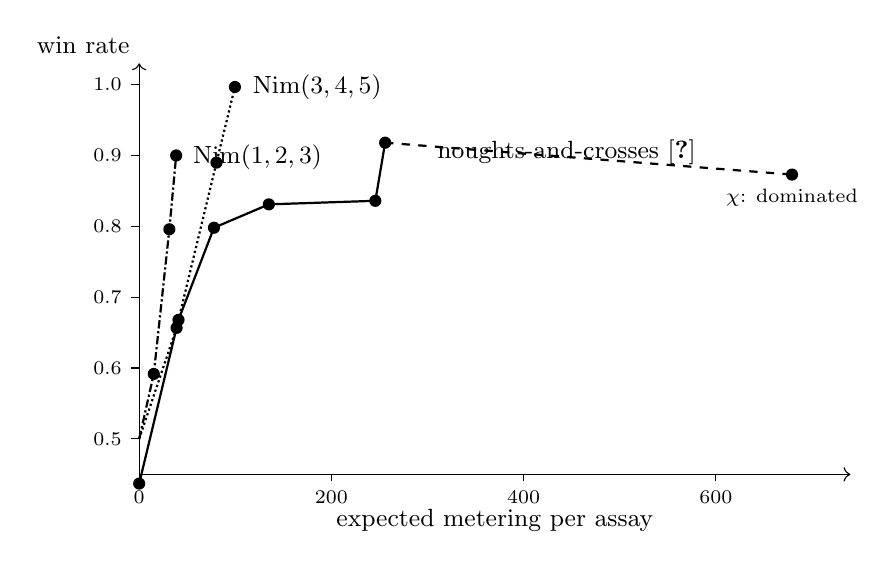
\begin{tikzpicture}[x=0.0122cm, y=9cm]
\draw[->] (0,0.45) -- (740,0.45);
\node[font=\small, below] at (370,0.415) {expected metering per assay};
\draw[->] (0,0.45) -- (0,1.03) node[above left, font=\small] {win rate};
\foreach \c in {0,200,400,600} \draw (\c,0.45) -- (\c,0.44) node[below, font=\scriptsize] {\c};
\foreach \w in {0.5,0.6,0.7,0.8,0.9,1.0} \draw (0,\w) -- (-8,\w) node[left, font=\scriptsize] {\w};
% noughts (from the game note)
\draw[thick] (0,0.437) -- (40.9,0.668) -- (77.8,0.798) -- (134.9,0.831) -- (245.7,0.836)
  -- (255.9,0.918);
\draw[thick, dashed] (255.9,0.918) -- (679.2,0.873);
\foreach \p/\l in {0/0.437, 40.9/0.668, 77.8/0.798, 134.9/0.831, 245.7/0.836, 255.9/0.918,
                   679.2/0.873} \fill (\p,\l) circle (2.2pt);
\node[font=\small, anchor=west] at (300,0.905) {noughts-and-crosses \cite{game}};
\node[font=\scriptsize, anchor=north] at (679.2,0.866) {$\chi$: dominated};
% nim 345
\draw[thick, densely dotted] (0,0.500) -- (38.9,0.6567) -- (80.4,0.8899) -- (99.6,0.9966);
\foreach \p/\l in {38.9/0.6567, 80.4/0.8899, 99.6/0.9966} \fill (\p,\l) circle (2.2pt);
\node[font=\small, anchor=west] at (108,0.9966) {Nim$(3,4,5)$};
% nim 123
\draw[thick, densely dashdotted] (0,0.500) -- (15.2,0.5917) -- (31.4,0.7958) -- (38.5,0.9000);
\foreach \p/\l in {15.2/0.5917, 31.4/0.7958, 38.5/0.9000} \fill (\p,\l) circle (2.2pt);
\node[font=\small, anchor=west] at (46,0.898) {Nim$(1,2,3)$};
\end{tikzpicture}
\caption{Three ladders on one pair of axes. The noughts-and-crosses curve turns down at its last
rung---the complete theory costs more and wins less than the heuristic beneath it. Both Nim
curves rise to the end, and the Nim$(1,2,3)$ curve rises fastest at the top. Composition puts
learners with curves of both shapes under one conserved $\Theta$.}
\label{fig:ladders}
\end{figure}

\subsection{The composite}

Let $\Lrn_A$ be a population playing noughts-and-crosses and $\Lrn_B$ a population playing
Nim$(1,2,3)$, each against the practice wall of~\cite[\S3.2]{game}, rooted at distinct quotations
so that Proposition~\ref{prop:root} applies. They share exactly the wall:
$\mathbf{k} = (0,1,0,0)$. The wall's reserve is $R_0 = 12{,}000$ at quantum $q = 6$, and the
price is $p = 0.05$ tokens per metered unit, as in that note's world.

At $p = 0.05$ and $q = 6$ a rung is self-funding exactly when its expected metering is below
$q/p = 120$. For the noughts ladder that admits rungs $0,1,2$ and excludes $3,4,5,6$; so
$\Lrn_A$'s deepest self-funding rung is rung 2, at $c_A = 77.8$ and a net of $+2.11$ tokens per
assay, and every deeper rung must be funded out of accumulated surplus. For $\Lrn_B$, $\chi_{\mathrm{Nim}}$
costs $c_B = 38.5$, net $+4.08$: \emph{the complete theory of $\Lrn_B$'s environment is
self-funding, and the incomplete theory of $\Lrn_A$'s environment is not.}

\begin{table}[t]
\centering
\small
\begin{tabular}{@{}lrrrr@{}}
\toprule
 & share of wall & assays & terminal surplus & rung-5 assays funded \\
\midrule
$\Lrn_A$ alone & $1.000$ & $2000$ & $4220$ & $621$ \\
$\Lrn_A$ composed & $0.331$ & $662$ & $1397$ & $206$ \\
$\Lrn_B$ composed & $0.669$ & $1338$ & $5452$ & --- (none needed) \\
\bottomrule
\end{tabular}
\caption{The composite, exactly. $\Lrn_A$ retains $0.331$ of the deep inquiry it could afford
alone---identically its share of the wall, per Proposition~\ref{prop:dilution}---and loses
$66.9\%$. $\Lrn_B$ loses $33.1\%$ of its assays and none of its depth, because the rung it holds
is self-funding. Neither learner perceives, models, or touches the other.}
\label{tab:composite}
\end{table}

\begin{observation}[The measurement]
$\Lrn_A$'s affordable depth falls from $621$ assays of rung-5 play to $206$. The mechanism is
entirely $\Theta$: $\Lrn_B$ holds no hypothesis about $\Lrn_A$, has no probe name in common with
it, could not derive its metabolic channel if it wanted to, and would gain nothing by doing so.
It simply finishes its assays faster, because its environment admitted a cheap complete theory,
and therefore reaches the wall more often.
\end{observation}

\begin{observation}[And it is regressive]
$\Lrn_B$ is unaffected in depth. Its best rung is self-funding, so the surplus it forgoes buys it
nothing it needs. $\Lrn_A$ is affected in depth alone, because everything it still wants to learn
runs a deficit. The learner with the finished science pays in currency it does not spend; the
learner with the unfinished science pays in the only currency that matters to it.
\end{observation}

\begin{figure}[t]
\centering
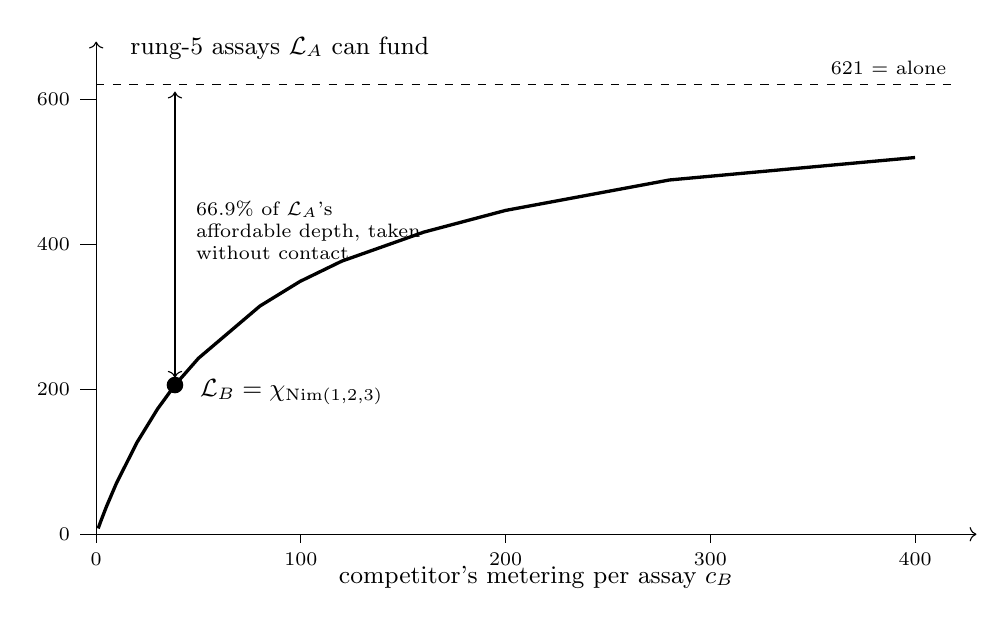
\begin{tikzpicture}[x=0.026cm, y=0.0092cm]
\draw[->] (0,0) -- (430,0);
\node[font=\small, below] at (215,-30) {competitor's metering per assay $c_B$};
\draw[->] (0,0) -- (0,680);
\node[font=\small, anchor=north west, align=left] at (12,700) {rung-5 assays $\Lrn_A$ can fund};
\foreach \c in {0,100,200,300,400} \draw (\c,0) -- (\c,-12) node[below, font=\scriptsize] {\c};
\foreach \d in {0,200,400,600} \draw (0,\d) -- (-8,\d) node[left, font=\scriptsize] {\d};
\draw[dashed] (0,621) -- (420,621);
\node[font=\scriptsize, anchor=south east] at (420,621) {$621$ = alone};
\draw[very thick] plot coordinates {
 (1,8) (2,16) (5,38) (10,71) (20,127) (30,173) (38.5,206) (50,243) (80,315) (99.6,349)
 (120,377) (160,417) (200,447) (280,489) (400,520)};
\fill (38.5,206) circle (3pt);
\node[font=\small, anchor=west] at (46,196) {$\Lrn_B = \chi_{\mathrm{Nim}(1,2,3)}$};
\draw[<->] (38.5,216) -- (38.5,611);
\node[font=\scriptsize, anchor=west, align=left] at (44,420) {$66.9\%$ of $\Lrn_A$'s\\affordable
depth, taken\\without contact};
\end{tikzpicture}
\caption{Competitive dilution. The curve is $D_A(c_B) = D_A^{\text{alone}} \cdot
c_B/(c_A + c_B)$ with $c_A = 77.8$, exactly as Proposition~\ref{prop:dilution} gives it. As the
competitor's science gets cheaper, the affordable depth of the learner whose science is still
unfinished goes to zero.}
\label{fig:dilution}
\end{figure}

\subsection{Succession is a change of the grading vector}

The wall is finite, so this composite has an ending, and the ending is where the typing of the
overlap earns its keep.

\begin{proposition}[Exhaustion forces a change of type]\label{prop:succession}
Let $\Lrn_1 \mid \Lrn_2$ have $\mathbf{k} = (0,1,0,0)$ with the shared source exhaustible. When
the source is exhausted, the foraging inequality fails at every source locus for both learners.
The composite then either dies or acquires $k_{\mathrm{met}} > 0$ or $k_{\mathrm{prb}} > 0$;
that is, succession in the sense of~\cite[Prop.~45]{scientist} is precisely a change in which
component of the grading vector is nonzero.
\end{proposition}

\begin{corollary}[The change is priced, and priced asymmetrically]
Acquiring $k_{\mathrm{met}} > 0$ requires deriving a name in the other learner's metabolic
namespace, which under capability gating is real work: a hypothesis describing that namespace
must be formed and installed as a guard. By Proposition~18 of~\cite{scientist} the branching a
learner can survey is its stack divided by the cost of one check. Hence the transition is
available to whichever learner retains apparatus for forming namespace hypotheses about adaptive
subjects---which by Corollary~42 there is the prey-feeder, and in this composite is the learner
whose science was unfinished.
\end{corollary}

In the worked composite, $\Lrn_B$ ends the source phase holding $5452$ tokens and $\Lrn_A$ holds
$1397$; $\Lrn_B$'s stack is $3.90$ times $\Lrn_A$'s. By the foraging inequality that stack is
worth opening at any concealment depth these prices make affordable. So the learner that was
confined during the source phase is the one positioned to harvest at succession, and the capital
it harvests was accumulated by the learner that confined it.

\begin{remark}[Offered as a structure, not a moral]
We resist reading anything edifying into this. What the framework says is narrow and checkable:
a cheap complete theory is a source-like access profile---non-adaptive, converged, with no
standing revision cost---and by Corollary~42 of~\cite{scientist} the apparatus for modelling
adaptive subjects is a heterotroph's expense, not carried by anything that does not need it. A
learner that has finished its science has, by construction, stopped paying for the machinery that
would let it form a hypothesis about a competitor. That is not a punishment for being right. It
is what being right in a closed domain costs, and it is the same fact as Proposition~32 of
\cite{game}: a solved science is a dead ecology.
\end{remark}

\section{The three units of learning}\label{sec:units}

Collecting the three notes, the units of learning are distinguished by exactly one thing: the
revision distance each can reach.

\begin{table}[h]
\centering
\small
\begin{tabular}{@{}llll@{}}
\toprule
unit & mechanism & reachable move & authority \\
\midrule
individual & walk the relaxation lattice & confined below $2^{-n}$ &
  \cite[Prop.~13]{scientist} \\
lineage & crossover at a shallow locus & $2^{-1}$ &
  \cite[\S12.10]{scientist}, \cite[\S9.3]{game} \\
composed learner & adopt another root & the whole tree &
  \S\ref{sec:comp}, Prop.~\ref{prop:root} \\
\bottomrule
\end{tabular}
\end{table}

\begin{proposition}[Composition reaches what no lineage reaches]
A lineage's recombination acts at loci of its own genomes, so every allele it can install already
occurs in one of its members and every namespace it can come to describe is generated from its own
root. Under Proposition~\ref{prop:root} a change of root is therefore unreachable by
recombination. It is reachable by composition, since $\Nsp_1 \vee \Nsp_2$ contains names
manufactured from both roots and the composite may install guards over either.
\end{proposition}

\begin{remark}[The series, and where it stops]
The game note measured the middle row: the corner-opening allele was unreachable to any
individual by deepening, free to a lineage by crossover, and the invasion was unconditional. The
top row is the analogue one step up, and its content is that whatever a lineage's early
commitments fixed---not merely its opening, but the family of names its whole hypothesis language
is generated from---is fixed for good against every mechanism internal to it. Composition is the
only operator in these notes that changes it, and merger (\S\ref{sec:merger}) is the only one
that changes the learner's identity along with it. We do not know whether the series continues,
and Problem~\ref{op:series} asks.
\end{remark}

\section{Composition is the exit from the dead ecology}

Proposition~32 of~\cite{game} says a population all of whose members hold theories that draw
against one another performs no harvest, burns tokens to live, and starves; and that the better
its science the sooner it dies. Remark~34 there lists three exits and takes none of them: enlarge
the game so $\chi$ is unaffordable, let the rules drift, or admit an external source.

The first exit is composition.

\begin{proposition}[Composition restores harvest]
Let $\Lrn$ be a learner in the terminal state of~\cite[Prop.~32]{game}: harvest rate zero,
$\chi$ held by every member, $\sigma$ declining monotonically. Let $\Lrn'$ be any learner whose
probe namespace is generated from a distinct root, so that $\Lrn$ holds no hypothesis satisfied
by $\Lrn'$'s components. Then in $\Lrn \mid \Lrn'$ with $k_{\mathrm{met}} > 0$ the foraging
inequality is satisfiable again, because $\Lrn'$'s stacks are concealed at a depth $\Lrn$ has not
paid to see, and paying is once more a purchase with a return.
\end{proposition}

\begin{remark}[Enlarging the game and composing are the same operation]
This is the content we would most like a reader to take away. ``Enlarge the game so that the
complete theory is unaffordable'' sounds like a modelling intervention---a change of domain
imposed from outside. Under Definition~\ref{def:comp} it is an operation \emph{inside} the
framework, performed by the ecology on itself, requiring no new rewrite rule and no new sort. A
science that has closed reopens by meeting a science that has not. The heat death of~\cite{game}
was never a property of noughts-and-crosses; it was a property of a world with one game in it.
\end{remark}

\section{What this shows, and what it does not}\label{sec:notshown}

\paragraph{Shown.}
That a learner may be taken to be a weighted population and hence a namespace, and that under
that reading composition is parallel composition on terms, disjunction on namespaces, and
undetermined on distributions (\S\ref{sec:learner}--\S\ref{sec:comp}). That disjointness of
namespaces is exactly factorisation of the distribution, so the lax comparison map's defect
\emph{is} the interaction and is a quantity rather than a caveat (Theorem~\ref{thm:factor},
Proposition~\ref{prop:lax}). That a typed grading vector recovers the ecological relations as
sign conditions (\S\ref{sec:typed}). That conservation makes epistemic overlap the only
positive-sum overlap (\S\ref{sec:coop}). That non-interference is unstable by default and
purchasable by rooting (\S\ref{sec:stability}). That phase is not compositional
(\S\ref{sec:phase}) and that competitive dilution confines a learner without contact, in a closed
form and on exact numbers (\S\ref{sec:dilution}--\S\ref{sec:worked}).

\paragraph{Not shown.}
We have not proved a monoidal-category theorem: Proposition~\ref{prop:lax} gives the comparison
map and its invertibility condition, and the coherence conditions, the unit laws up to the
identifications merger imposes, and the relationship to the fibration's section are left open.
Definition~\ref{def:rate} is a modelling choice; under the round-robin alternative each learner
receives half the payouts and the retained fraction becomes $1/2$ for both, so the
\emph{dilution} survives and the \emph{regressiveness} weakens to whatever asymmetry the rungs
themselves carry---in the worked composite $\Lrn_A$ would retain $0.500$ rather than $0.331$, and
still lose depth where $\Lrn_B$ loses none. As in~\cite{game} the measurements are exact
computations over policies rather than observations of a running population: the ecology of
Appendix~\ref{app:world} is written and not run to a fixed point, so every claim about invasion
and succession is a claim about payoffs. And the Nim ladders, like the noughts ladder, are
priced by a schedule that is a choice.

\paragraph{The honest summary.}
The composition operator was, going in, an obvious formality---parallel composition is already
there, and saying that learners compose by it looks like a restatement. What the exercise
produced instead was three things we did not put in: that the probabilistic content of
composition is exactly a graded separation, that a typed grading vector is forced rather than
convenient, and that two learners which cannot perceive each other can nonetheless confine each
other's inquiry by a measurable amount.

\section{Open problems}

\begin{enumerate}[itemsep=4pt]
\item \textbf{Coherence.} Is $(\mathrm{Eco}, \mid, \mathbf{0})$ lax monoidal with
$\lambda$ of Proposition~\ref{prop:lax} as the structure map, and is the canonical section of
\cite[Prop.~80]{scientist} lax monoidal over it? The obstruction to strictness is located; the
coherence conditions are not checked.

\item \textbf{Is the grading vector complete?} Definition~\ref{def:typed} gives four
sub-namespaces because four are what the companion notes distinguish. Is there a fifth? The
candidate is the \emph{arena} namespace: the names by which an admitted context class
$\mathcal{A}$ is realised (\cite[Obs.~4]{game}). Two learners sharing an arena but no other name
play the same game against different opponents, which is neither of the relations in
Table~\ref{tab:relations}.

\item \textbf{Optimal $\mathbf{k}$.} Given a distribution over environments, is there an optimal
grading vector for a learner to hold---an amount of overlap that maximises expected residual
life? \S\ref{sec:coop} says the $\Prb$ component should be positive and the $\Met$ component
should be zero or pooled, but the trade-off against the exposure of Lemma~33
of~\cite{scientist} is not worked.

\item \textbf{Run the composite.} Appendix~\ref{app:world} specifies a two-learner world;
\S\ref{sec:worked} computes payoffs. Sampling trajectories by the Gillespie construction
of~\cite{gillespie-note} would turn Table~\ref{tab:composite} from a payoff calculation into an
ensemble result, and would settle whether the succession of Proposition~\ref{prop:succession}
actually occurs or whether $\Lrn_A$ starves first.

\item \textbf{The plagiarism equilibrium, now well posed.} Problem~2 of~\cite{scientist} asked
whether honest science survives theory theft. With the grading vector it becomes: for which
$k_{\mathrm{prb}}$ is the two-way reading equilibrium stable against a one-way reader, and does
the answer depend on the shape of the ladder (Observation~\ref{obs:env}) in each learner's
environment?

\item \textbf{Does the series continue?}\label{op:series} Individual, lineage, composite: each
reaches a revision the one below cannot. Is there a fourth unit, and if so what does it reach?
The natural candidate is a distribution over \emph{composites}---a distribution over grading
vectors rather than over configurations---and we do not know whether that is a new object or the
same one at a coarser resolution.

\item \textbf{Cheapness versus completeness.} Observation~\ref{obs:env} shows that whether $\chi$
is a good purchase varies by environment. Is there a criterion---presumably in terms of Remark~11
of~\cite{scientist}, how much of the environment's regularity is structural, together with the
branching factor---that predicts the shape of the ladder without computing it? For a composite
this would predict who dilutes whom in advance of any measurement.
\end{enumerate}

\appendix

\section{A composite world, in rholang}\label{app:world}

The listing below is the composite of \S\ref{sec:worked}: two learners rooted at distinct
quotations, sharing exactly one source name, with the typed namespaces of
Definition~\ref{def:typed} written as name predicates and the grading vector as a family of
graded separations over them. Guards using a structural or modal connective are marked
\texttt{//!\ ideal} and specify a check rather than perform one; everything else runs.
Conservation is auditable by inspection: \texttt{Wall}, \texttt{Harvest} and \texttt{Beget} move
tokens, \texttt{Live} debits them, and nothing mints.

\begin{lstlisting}
// ============================================================================
// TWO LEARNERS, ONE WALL
// ============================================================================
//
// Companion listing to "Composing Learners".  The world is literally
//
//     Wall  |  L_A  |  L_B
//
// and every claim of the note is a claim about what that bar does.
//
// ROOTING (Prop. "Rooting makes disjointness a theorem").  Each learner
// manufactures every private name by quoting a term containing its OWN root.
// L_A's names are @[*rootA, ...] and L_B's are @[*rootB, ...].  By freshness-
// by-quotation no name of one is structurally equal to a name of the other,
// so k = 0 holds on every component of the grading vector EXCEPT the wall,
// whose name neither learner manufactured and both were handed.  That single
// imported name is the whole of the coupling.
//
// TYPED NAMESPACES (Def. "Typed namespaces").  Four predicates per learner:
//
//   Met(r) := @[ *r, "m", _ ]      metabolic: where stacks rest
//   Src(r) := @[ *r, "s", _ ]      source: emitters drawn upon
//   Prb(r) := @[ *r, "p", _ ]      probe: where assays are installed
//   Mat(r) := @[ *r, "g", _ ]      mating: where genomes are disclosed
//
// The grading vector of the composite is then the four-tuple
//
//   k_tau = | fn(L_A) /\ fn(L_B) /\ N_tau |
//
// and the note's claim is that this world has k = (0,1,0,0).

new stdout(`rho:io:stdout`), display, wall, rootA, rootB,
    Live, Wall, Assay, Ladder, Body, Harvest, Beget, Merge, Learner
in {

  for (@line <= display) { stdout!(line) }

  // ==========================================================================
  // METABOLISM.  Reclaim - debit - reissue.  Between the receipt and the send
  // the stack is a message in flight, which is what Harvest exploits.
  // ==========================================================================
  | contract Live(m, @burn, step) = {
      for (@sigma <- m) {
        match sigma > burn {
          true  => { m!(sigma - burn) | *step | Live!(*m, burn, *step) }
          false => { display!(("DIED", "could not fund a step")) }
        }
      }
    }

  // ==========================================================================
  // THE SHARED SOURCE.  One contract, hence rate-limited; non-exclusive, since
  // anyone holding the name may call it; non-adaptive; and finite.
  //
  // This contract IS the entire overlap.  Note what it does NOT do: it does
  // not know who is calling, does not adapt to callers, and cannot be used by
  // one caller to observe another.  Competitive dilution is delivered by a
  // process with no model of anybody.
  // ==========================================================================
  | contract Wall(w, @quantum, @reserve) = {
      for (ret <- w) {
        match reserve >= quantum {
          true  => { ret!(quantum) | Wall!(*w, quantum, reserve - quantum) }
          false => { ret!(0)       | Wall!(*w, quantum, 0) }   // exhausted
        }
      }
    }

  // ==========================================================================
  // THE ASSAY.  Unchanged from the companion notes: the hypothesis sits in
  // GUARD position, so playing IS testing and confirmation IS the rendezvous.
  // The probe name is manufactured from the learner's own root, which is why
  // k_prb = 0 -- neither learner can install a guard that the other's activity
  // could ever satisfy, because the names do not meet.
  // ==========================================================================
  | contract Assay(r, @g, @hyp, ret) = {
      new probe in {
        @[*r, "p", g]!(*probe)                     // probe in Prb(r)
        | wall!(*probe)                            // the ONE shared name
        //! ideal: structural guards
        | for (@pos <- probe where pos |= hyp)    { ret!(("confirm", pos)) }
        | for (@pos <- probe where ~(pos |= hyp)) { ret!(("refute",  pos)) }
      }
    }

  // ==========================================================================
  // THE LADDERS.  Two environments, two shapes.  L_A's ladder is the
  // noughts-and-crosses ladder of the game note: chi is dominated and every
  // rung above 2 runs a metabolic deficit at the wall's quantum.  L_B's is the
  // Nim ladder: chi_Nim is a NAME-LEVEL predicate of depth zero, so the
  // complete theory of L_B's environment is self-funding.
  //
  //! ideal throughout.
  // ==========================================================================
  | contract Ladder(@which, @r, ret) = {
      match (which, r) {
        // -- L_A: noughts-and-crosses, costs 0 / 40.9 / 77.8 / ... / 679.2
        ("ttt", 2) => { ret!( @{ exists s. Emp(s) and
                                 (Thr(s, me) or Thr(s, them)) } ) }
        ("ttt", 5) => { ret!( @{ exists s. Emp(s) and
                                 (Thr(s, me) or Thr(s, them))
                                 or <<K s>> Fork(me)
                                 or forall t. <<K s>>[K t] ~Fork(them)
                                 or Central(s) } ) }
        ("ttt", 6) => { ret!( @{ nu X. forall s.
                                 [K s]( ~Lost and exists t. <<K t>> X ) } ) }
        // -- L_B: Nim.  Note the absence of any modality anywhere.
        ("nim", 1) => { ret!( @{ exists s. One and Takes(s) } ) }
        ("nim", 2) => { ret!( @{ exists s. (One and Takes(s))
                                 or (Two and Equalises(s)) } ) }
        ("nim", 3) => { ret!( @{ exists s. (One and Takes(s))
                                 or (Two and Equalises(s))
                                 or NimSumZero(s) } ) }        // chi_Nim
      }
    }

  // ==========================================================================
  // A LEARNER.  Not a scientist: a POPULATION, rooted, weighted by the stacks
  // its members hold.  What makes it one learner rather than several is the
  // root, which is what its whole namespace is generated from.
  // ==========================================================================
  | contract Learner(r, @which, @rung, @burn, @members) = {
      match members {
        [] => { Nil }
        [h ...t] => {
            Body!(*r, which, rung, burn, h)
          | Learner!(*r, which, rung, burn, t)
        }
      }
    }

  | contract Body(r, @which, @rung, @burn, @i) = {
      new hyp, score in {
          @[*r, "m", i]!(400)                       // the stack: in Met(r)
        | score!(0, 0)
        | Ladder!(which, rung, *hyp)
        | Live!(@[*r, "m", i], burn, @{
              new ret in {
                  for (@h <- hyp) { hyp!(h) | Assay!(*r, i, h, *ret) }
                | for (@o <- ret) {
                    for (@c, @f <- score) {
                      match o {
                        ("confirm", q) => { score!(c + 1, f)
                                            | for (@s <- @[*r,"m",i]) {
                                                @[*r,"m",i]!(s + q) } }
                        _              => { score!(c, f + 1) }
                      }
                    }
                  }
              }
          })
      }
    }

  // ==========================================================================
  // SUCCESSION.  When the wall returns 0 forever, the only credit left is in
  // another learner's Met namespace -- which is a namespace this learner has
  // never described, because k_prb = 0 kept it invisible.  Acquiring it is a
  // step, and the step is metered: a hypothesis over Met(rOther) must be
  // formed and installed.  That is the change of grading vector, and it is
  // available only to a learner that still carries the apparatus.
  // ==========================================================================
  | contract Harvest(@rSelf, @i, @rOther, ret) = {
      //! ideal -- the guard is a name predicate over the OTHER root's
      // metabolic namespace.  Forming it is what costs; firing it is a comm.
      for (@mPrey <- @[*rSelf, "p", "hunt"]
             where mPrey |= @{ Met(rOther) }) {
        for (@sigma <- @{mPrey}) {
          for (@own <- @[*rSelf, "m", i]) {
              @[*rSelf, "m", i]!(own + sigma)
            | ret!(("harvest", sigma))
            | display!(("HARVEST across roots", sigma))
          }
        }
      }
    }

  | contract Beget(m, @alleles, @endow, ret) = {
      for (@sigma <- m where sigma > endow + 40) {
          m!(sigma - endow)
        | match alleles {
            [w, rg] => {
              new childM, code in {
                  code!( @{ Body!(*childM, w, rg, 2 + rg, endow) } )  // inert
                | for (g <- code) { *g | childM!(endow) }             // metered
                | ret!(("born", w, rg))
              }
            }
          }
      }
    }

  // ==========================================================================
  // MERGER -- a DIFFERENT OPERATOR, and this is the point of the section.
  //
  // Composition is the bar.  It is free, it is associative and commutative,
  // and it leaves both learners identifiable afterwards.  Merger identifies
  // the two MATING namespaces, which is a step, is metered, and is
  // irreversible: after it there is no composition recovering the parts,
  // because alleles have crossed roots.
  //
  // Note that Merge is a CONTRACT and `|` is not.  That asymmetry is the
  // formal content of "merger is a separate operator".
  // ==========================================================================
  | contract Merge(@rA, @rB, ret) = {
      new rC in {
          // the merged learner's mating namespace admits homologous loci
          // across BOTH roots; this identification is what cannot be undone
          @[*rC, "g", "admits"]!([rA, rB])
        | ret!(*rC)
      }
    }

  // ==========================================================================
  // THE WORLD.   Theta = 12000 (wall) + 3 x 400 (L_A) + 3 x 400 (L_B) = 14400.
  //
  // The composite is the bar between the two Learner calls.  Delete either and
  // the other's numbers change -- by exactly the factor of Prop. "competitive
  // dilution", and by nothing else, since no other name is shared.
  // ==========================================================================
  | Wall!(*wall, 6, 12000)

  | Learner!(*rootA, "ttt", 2, 4, [0, 1, 2])   // noughts: rung 2, c = 77.8
  | Learner!(*rootB, "nim", 3, 5, [0, 1, 2])   // nim: chi_Nim, c = 38.5

  // --------------------------------------------------------------------------
  // WHAT TO WATCH
  //
  // * The overlap is ONE NAME.  `wall` is the only identifier appearing in
  //   both Learner subtrees.  Everything else is manufactured under a root.
  //   k = (0,1,0,0), and it stays there by construction, not by luck.
  //
  // * Nobody models anybody.  No guard anywhere mentions the other root.
  //   L_B has no hypothesis about L_A and would gain nothing from one.  The
  //   dilution happens anyway.
  //
  // * L_B finishes and L_A does not.  L_B holds the complete theory of its
  //   environment at burn 5; L_A holds an incomplete one at burn 4 and cannot
  //   afford the rungs it still wants.  The one still climbing is the one the
  //   competition costs.
  //
  // * And it ends.  When the wall returns 0, Assay's confirm guard stops
  //   crediting, Live keeps debiting, and the only remaining credit is inside
  //   the other root's Met namespace.  Reaching it is Harvest, and Harvest's
  //   guard is a hypothesis somebody has to be able to afford to form.
  // --------------------------------------------------------------------------
}
\end{lstlisting}

\section{Reproducing the numbers}\label{app:repro}

All figures in \S\ref{sec:worked} are exact computations, not samples. The noughts-and-crosses
ladder figures---win rates $0.437$, $0.668$, $0.798$, $0.831$, $0.836$, $0.918$, $0.873$ and
expected meterings $0.0$, $40.9$, $77.8$, $134.9$, $245.7$, $255.9$, $679.2$---are quoted from
Table~1
of~\cite{game} and were not recomputed here.

The Nim ladders are computed by \texttt{compose.py}, which enumerates positions as sorted tuples
of heap sizes, evaluates each rung by memoised recursion over all plays with uniform tie-breaking
within a rung and a uniform-random opponent, and charges $|M| \cdot \sum_{1..r} \kappa$ at each
decision of the policy player with $\kappa(d) = 2^d$ and depths $1, 1, 0$ for the three rules.
Probabilities are carried as exact rationals and converted to decimal only for display. Figures
are symmetrised over which side moves first; the unsymmetrised figures are reported separately
where the colour asymmetry is the point.

The composite of \S\ref{sec:worked} uses $R_0 = 12{,}000$, $q = 6$, $p = 0.05$, shares by
Definition~\ref{def:rate}, and the identity of Proposition~\ref{prop:dilution}; the
computation is a few lines and is included in the same script for auditability rather than for
difficulty.

\begin{thebibliography}{99}

\bibitem{scientist} L. G. Meredith. \emph{The Mortal Scientist: learning as cost-accounted
computation in a reflective higher-order calculus.} F1R3FLY.io, 2026.

\bibitem{game} L. G. Meredith. \emph{Learning to Play: noughts-and-crosses as an ecology of
mortal scientists.} F1R3FLY.io, 2026.

\bibitem{classifier} L. G. Meredith. \emph{Classifying knot diagrams with a spatial--behavioural
logic: a logic obtained for free from the encoding of knots as processes.} F1R3FLY.io, 2026.

\bibitem{knots} L. G. Meredith. \emph{Knots as cost-accounted rholang processes: a
Dowker--Thistlethwaite-driven encoding and weak-bisimulation invariance.} F1R3FLY.io, 2026.

\bibitem{gslt} \emph{Graph-structured lambda theories: a reference for the working developer.}
F1R3FLY.io, 2026.

\bibitem{universality} L. G. Meredith. \emph{Probing universality: context-labelled bisimulation
and a relative refinement of Turing completeness for interactive GSLTs.} F1R3FLY.io, 2026.

\bibitem{gillespie-note} L. G. Meredith. \emph{Stochastic simulation for decorated ciGSLTs.}
F1R3FLY.io, 2026.

\bibitem{nslogic} L. G. Meredith and M. Radestock. Namespace logic: a logic for a reflective
higher-order calculus. In \emph{Trustworthy Global Computing}, LNCS 3705, Springer, 2005.

\bibitem{rho} L. G. Meredith and M. Radestock. A reflective higher-order calculus.
\emph{Electronic Notes in Theoretical Computer Science} 141(5):49--67, 2005.

\bibitem{caires} L. Caires and L. Cardelli. A spatial logic for concurrency (part I).
\emph{Information and Computation} 186(2):194--235, 2003.

\bibitem{bouton} C. L. Bouton. Nim, a game with a complete mathematical theory.
\emph{Annals of Mathematics} 3(1/4):35--39, 1901--1902.

\bibitem{onag} J. H. Conway. \emph{On Numbers and Games.} Academic Press, 1976.

\bibitem{hardin} G. Hardin. The competitive exclusion principle. \emph{Science}
131(3409):1292--1297, 1960.

\bibitem{tilman} D. Tilman. \emph{Resource Competition and Community Structure.} Princeton
University Press, 1982.

\bibitem{margulis} L. Margulis. \emph{Origin of Eukaryotic Cells.} Yale University Press, 1970.

\bibitem{smith} E. Smith and H. J. Morowitz. \emph{The Origin and Nature of Life on Earth: The
Emergence of the Fourth Geosphere.} Cambridge University Press, 2016.

\bibitem{gillespie} D. T. Gillespie. Exact stochastic simulation of coupled chemical reactions.
\emph{Journal of Physical Chemistry} 81(25):2340--2361, 1977.

\end{thebibliography}

\end{document}
